%
%%
%%
%%

%% [intro]

The calibration of the instrument NIKA2 in its final configuration
of January 24th 2017  is studied in this section  in using the 
 primary calibrators, Uranus and Neptune, and secondary calibrators ; the two largest asteroids Ceres and Vesta, and the three
planetary nebulae NGC7027, CRL2688, and MWC349.

% HA 
\subsection{NIKA2 Photometric System}


\begin{table}[h]
\begin{center}
\begin{tabular}{|c|c|c|}
\hline
     & 1mm & 2mm \\
\hline
Reference frequency $\nu_{0}$ & 260 GHz & 150 GHz \\
\hline
Reference FWHM                      & 12.5  '' & 18.5 '' \\
\hline
\end{tabular}
\caption{NIKA2 reference frequencies and FWHM}
\end{center}
\label{tab:definitions}
\end{table}

\subsubsection{Response of a detector to astronomical source}


Let us consider a source observed at airmass $\sec z$ under
$mm_{H_{2}O}$ of precipitable water, with specific intensity $I_{\nu}$ (in units
of  $W/m^{2}/sr/Hz$) in the direction $\theta, \phi$, where $\theta$
is the off-axis distance and $\phi$ the position angle, illuminating a KID
of the NIKA2 array. 

A KID response located at position $\theta, \phi$
on the focal plane to this signal will be:
\begin{equation}
R(\theta, \phi, \sec z, mm_{H_{2}O}) = G_{k} \int_{0}^{+\infty} I(\nu)
\frac{T'(\nu)}{\left(\frac{\nu}{\nu_{0}}\right)^{2}} e^{\left(-\sec z
  . \tau(\nu,  mm_{H_{2}O})\right)}A\Omega (\nu)  d\nu 
\label{eq:basicphot}
\end{equation}

where the different factors in the integral are:
\begin{itemize}
\item $\frac{T'(\nu)}{\left(\frac{\nu}{\nu_{0}}\right)^{2}}$:  the
  system transmission. $T'(\nu)$ is the transmission as measured in
  section~\ref{se:bandpasses} with a Rayleigh-Jeans source. It is
  divided by $\left(\frac{\nu}{\nu_{0}}\right)^{2}$ to correct for the
  incident spectrum.
\item $e^{\left(-\sec z . \tau(\nu,  mm_{H_{2}O} )\right)}$: the
  atmospheric transmission at airmass  $\sec z$ for an amount of
  precipitable water vapor $mm_{H_{2}O}$ generating an opacity $\tau(\nu)$.
\item $A\Omega (\nu) $: the KID etendue, {\it i. e.} the product of
  its light collecting area by the solid angle it intercept on the
  sky. While the step between  pixels is well known and is measured (see sec~\ref{se:fov}), the
  actual solid angle is not known precisely and is {\em probably} a function of the
  frequency  because the pixels sizes are close to the wavelength of
  operation (2.75 mm at 2mm for example). The collecting $A$ area is the
  projection of the IRAM primary on the cold pupil and is also not
  known very accurately.
\end{itemize}
The integral in eq~\ref{eq:basicphot} gives the total power (units of $W$)
falling on a pixel. The factor $G_{k}$ (units of  $W^{-1}$) convert this
power to ADU. 

By virtue of the conservation of specific intensity in a telescope,
equation~\ref{eq:basicphot} can be rewritten as:
\begin{equation}
R(\theta, \phi, \sec z, mm_{H_{2}O}) = G_{k} A_{pupil}\Omega_{s}\int_{0}^{+\infty} I(\nu)
\frac{T'(\nu)}{\left(\frac{\nu}{\nu_{0}}\right)^{2}} e^{\left(-\sec z
  . \tau(\nu,  mm_{H_{2}O})\right)} \Omega_{beam} (\theta, \phi, \nu)  d\nu 
\label{eq:basicphot2}
\end{equation}
where:
\begin{itemize}
\item $A_{pupil}$ is the area of the entrance pupil ({\it i.e.} the
  dish collecting area).
\item $\Omega_{s}$ is the solid angle of the source seen from the
  entrance pupil.
\item $\Omega_{beam}(\theta, \phi, \nu)$ is the fraction of source signal
  illuminating the KID. It has no units and it is thus normalized so that:
\begin{equation}
\int\int_{4\pi} \Omega_{beam}(\theta, \phi, \nu) \sin \theta d\theta
d\phi = 1 
\label{eq:omegabdef}
\end{equation}
\end{itemize}

Equation~\ref{eq:basicphot2} describe the response of a KID, and it
is quite complex. We will in the following simplify it by making a few
assumptions. Let us first turn ourselves toward the effect of the
atmosphere. 


\subsubsection{Effect of the atmosphere}

In order to study the effects of the atmosphere, let us define the
effective frequency of a source as the weighted frequency of the
passband, taking into account the system and atmospheric transmission,
as well as the shape of the incident spectrum:
\begin{equation}
\nu_{eff}( \sec z, mm_{H_{2}O}) = \frac{ \int_{0}^{+\infty} I(\nu) \frac{T'(\nu)}{\left(\frac{\nu}{\nu_{0}}\right)^{2}} e^{\left(-\sec z
  . \tau(\nu,  mm_{H_{2}O})\right)} \nu d\nu } { \int_{0}^{+\infty} I(\nu) \frac{T'(\nu)}{\left(\frac{\nu}{\nu_{0}}\right)^{2}} e^{\left(-\sec z
  . \tau(\nu,  mm_{H_{2}O})\right)}  d\nu}
\label{eq:nueff}
\end{equation}
In order to compute the atmospheric tramission, we have used
the IRAM atmosphere 2009 models provided in GILDAS, computed for
'midlatwinter' conditions, a temperature of 268 K  and a pressure of 703.5
hPa. $\nu_{eff}$ allows to characterise the impact of the variation of
the atmospheric transmission on the full system transmisison.  Note
that the instrument transmission $T'(\nu)$ is the one measured in
sec~\ref{se:bandpasses}. 

Figure~\ref{fig:nueff} shows the variations of
$\nu_{eff}$ as a function of the water content of the atmosphere for
two elevations (zenith and 20 degree) and two spectral shape (RJ and
flat spectrum), in the two 1mm passbands and in the 2mm passband. 

Typical variations of $\nu_{eff}$ with the spectral shape of the
source range between 1\% and 3\%, and are relatively stable between good
($\tau_{225GHz} \simeq 0.1$) and
poor  ($\tau_{225GHz} \simeq 1.0$) atmospheric conditions for both the
1mm and 2mm bands. 


Let us now examine the effect of elevation.
Under good atmospheric conditions ($\tau_{225GHz} \simeq 0.1$), $\nu_{eff}$ change by
less than 0.3\% betwen zenith and 20 degree elevation. Under poor
conditions ($\tau_{225GHz} \simeq 1.0$), this rises to almost 3\% for
a Rayleigh-Jeans spectrum in the 2mm band, {\it i.e.} larger than the
  variations due to the spectral shape of the source.



\begin{figure}[h]
\begin{tabular}{cc}
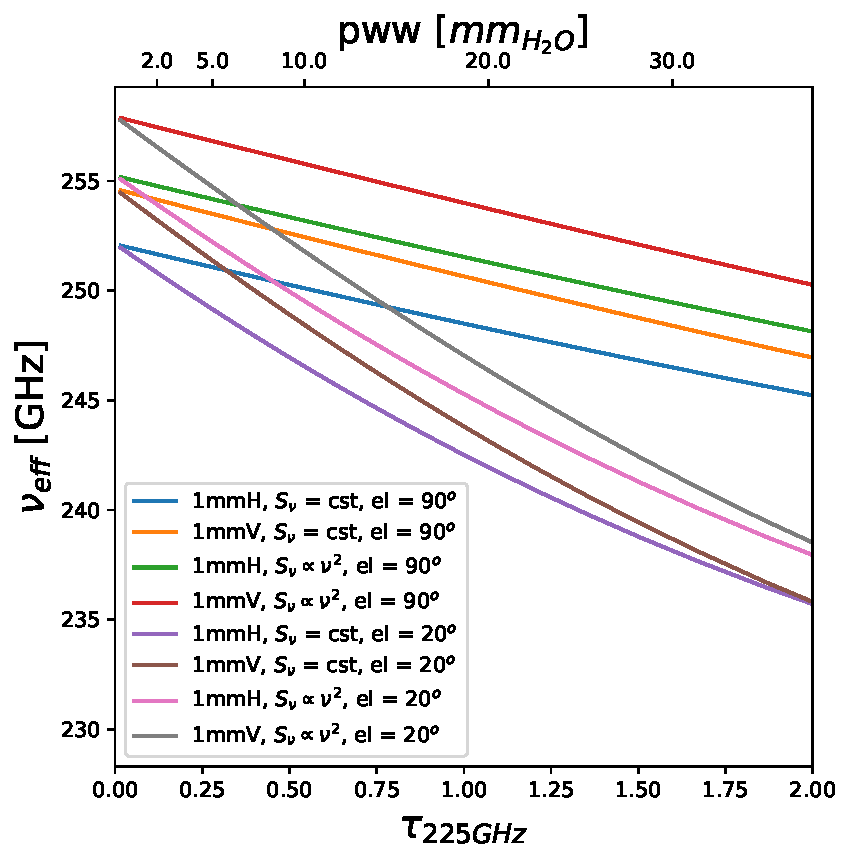
\includegraphics[width=0.5\textwidth]{Figures/atm_nueff_1mm.pdf}
  & 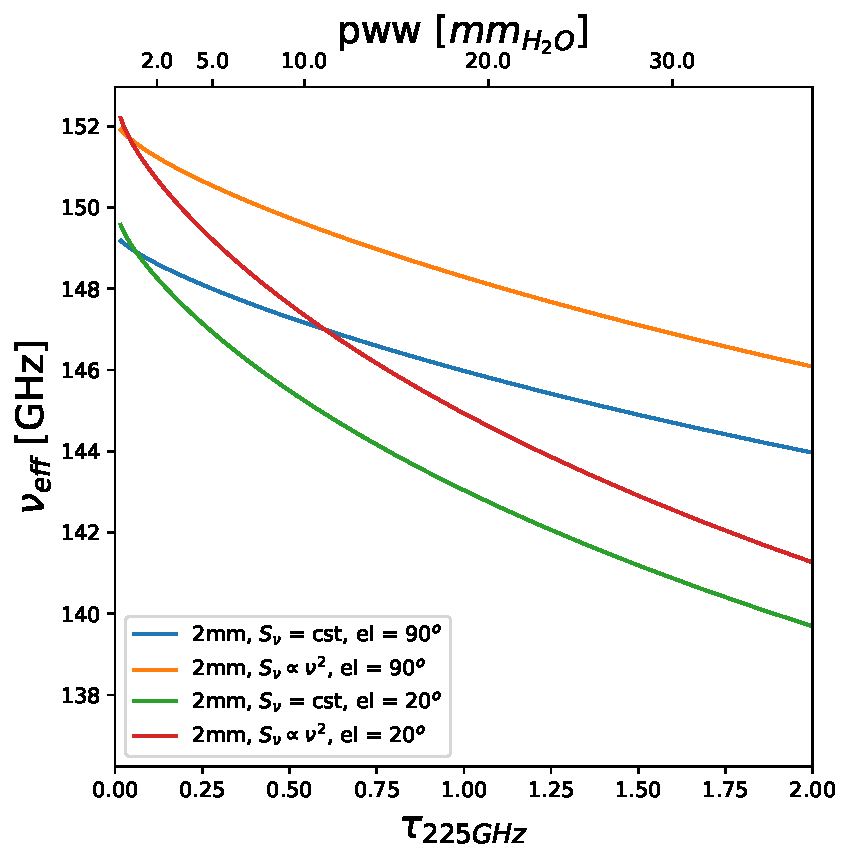
\includegraphics[width=0.5\textwidth]{Figures/atm_nueff_2mm.pdf}
  \\
a) 1mm & b) 2mm \\
\end{tabular}
\caption{Effective frequency as a function of the sky opacity. The
  effective frequency (see text) have been computed for two source
  spectra (RJ and constant), and for two elevations.}
\label{fig:nueff}
\end{figure}

Nevertheless, to a first approximation, we consider the shape of the atmospheric
transmission independent of the elevation and water content, so that  an
effective zenith opacity $\tau_{eff}$
used. 
Equation~\ref{eq:basicphot2} becomes under this assumption: 
\begin{equation}
R(\theta, \phi, \sec z, mm_{H_{2}O}) \simeq G_{k}  A_{pupil}\Omega_{s} e^{\left(-\sec z
  . \tau_{eff}(mm_{H_{2}O})\right)} \int_{0}^{+\infty} I(\nu)
\frac{T'(\nu)}{\left(\frac{\nu}{\nu_{0}}\right)^{2}} T_{atm}(\nu)
\Omega_{beam} (\theta, \phi, \nu) d\nu 
\label{eq:basicphot3}
\end{equation}
where $T_{atm}(\nu)$ is the transmission of the atmosphere at zenith,
and is a function of the frequency only. From the computations made to
plot figure~\ref{fig:nueff}, we derive that this approximation 
is valid below the percent level for $\tau_{225GHz} < 0.35$

The dependance on elevation and opacity can be corrected as shown in
section~\ref{se:skydip}, so that a response outside of atmosphere (in
terms of airmass, but not in terms of transmission) can be derived:
\begin{equation}
R(\theta, \phi) \simeq G_{k}  A_{pupil}\Omega_{s} \int_{0}^{+\infty} I(\nu)
\frac{T'(\nu)}{\left(\frac{\nu}{\nu_{0}}\right)^{2}} T_{atm}(\nu) \Omega_{beam} (\theta, \phi, \nu)  d\nu 
\label{eq:basicphot4}
\end{equation}
Equation~\ref{eq:basicphot4} is the main photometric equation.

Because both $A_{pupil}$ and $ \Omega_{beam} $ are not known with good
accuracy, it is not possible to compute all the terms of
eq.~\ref{eq:basicphot4} from first principles, and a practical way of
calibrating the system must be used: it is done by observing a primary
calibrator.

\subsection{Beammap of a calibrator}

A primary calibrator is a source whose spectral irradiance is
known. For NIKA2, we use two planets as primary calibrators, Uranus
and Neptune.



The specific intensity $I_{c}(\nu)$ of the
calibrator is:
\begin{equation}
I_{c}(\nu) =  \frac{S_{c}(\nu)}{\Omega_{s}} =\frac{ S_{c}
(\nu_{0})}{\Omega_{S}} f(\frac{\nu}{\nu_{0}})  
\end{equation}
Where $S_{c}(\nu)$ is the spectral irradiance of the calibrator (units
of $W/m^{2}/Hz$) or Jy. We parametrize the source spectral irradiance
as a function of a reference frequency $\nu_{0}$ that we choose
arbitrarily to be: $\nu_{0} = 150$~GHz for the 2mm array and $\nu_{0}
= 260$~GHz for both 1mm arrays. 


Equation~\ref{eq:basicphot4} becomes:
\begin{equation}
R(\theta, \phi) \simeq G_{k}  A_{pupil}  S_{c} (\nu_{0}) \int_{0}^{+\infty} f(\frac{\nu}{\nu_{0}})  
\frac{T'(\nu)}{\left(\frac{\nu}{\nu_{0}}\right)^{2}} T_{atm}(\nu) \Omega_{beam} (\theta, \phi, \nu)  d\nu 
\label{eq:basicphot5}
\end{equation}

Let further parametrize the beam as a function
of the effective frequency as defined in eq~\ref{eq:nueff},
considering that its frequency dependency is only due to the diffrection law,
hence a variation as $1/\nu$.

With this in hand, we can write the equation of a beammap using a
single KID with eq~\ref{eq:basicphot3}. At each position ($\theta,
\phi$) on the beam map we have:
\begin{equation}
R_{c}(\theta, \phi) =  G_{k} A_{pupil} S_{c} (\nu_{0})  \int_{0}^{+\infty}
f(\frac{\nu}{\nu_{0}}) \Omega_{b}(\nu_{0}, \theta \times \frac{\nu}{\nu_{0}},
\phi) \frac{T'(\nu)}{\left(\frac{\nu}{\nu_{0}}\right)^{2}}
T_{atm}(\nu) d\nu
\label{eq:beammap}
\end{equation}

\subsection{Calibration in FWHM$_{0}$ beam}

This map is fitted with au gaussian of fixed width: FWHM$_{0}$ (we
recall that $2 \sqrt{2\ln{2}} \sigma_{0} =  FWHM_{0}$).
\begin{equation} 
R_{c}(\theta, \phi) = \frac{A_{c}}{2 \pi \sigma_{o}^{2}}
e^{-\frac{\theta^{2}}{2\sigma_{0}^{2}}}  + \epsilon(\theta, \phi)
\end{equation}
where $\epsilon(\theta, \phi)$ are the residuals of the fit.

Assuming that the fit is not biased, we have:
\begin{equation} 
\int\int R_{c}(\theta, \phi) d\theta d\phi = A_{c}
\end{equation}
because errors average out so that:
\begin{equation} 
\int\int \epsilon (\theta, \phi) d\theta d\phi = 0
\end{equation}
But we also know that integral of the beammap should give the power
emitted by the source. Therefore we form the map:
\begin{equation}
M_{c}(\theta, \phi) = R_{c}(\theta, \phi)   S_{c} (\nu_{0}) / A_{c}
\end{equation}
Where  $S_{c} (\nu_{0})$ is the spectral irradiance of the calibrator
at a reference frequency $\nu_{0}$ given in
table~\ref{tab:definitions}. This map has units of $W/m^{2}/Hz$. Note
that the choice of the reference frequency is arbitrary, it is a
convention. By construction, integrating over the map we have:

\begin{equation}
\int\int M_{c}(\theta, \phi) d\theta d\phi = S_{c}(\nu_{0})
\end{equation}



Similarly, a point source with spectral irradiance $S_{s}(\nu)$ will
generate a response at position $(\theta, \phi)$
\begin{equation}
R_{s}(\theta, \phi) =  G_{k} A_{pupil}  \int_{0}^{+\infty}
S_{s}(\nu) \Omega_{b}(\nu_{0}, \theta \times \frac{\nu}{\nu_{0}},
\phi) \frac{T'(\nu)}{\left(\frac{\nu}{\nu_{0}}\right)^{2}}
T_{atm}(\nu) d\nu
\end{equation}
Note here that the effective frequency for the beam is not necessarily
the same as the one for the primary calibrator, as it depends on the
source spectrum.


This beammap will be fitted with a gaussian of fixed width:
\begin{equation} 
R_{s}(\theta, \phi)  = \frac{A_{s}}{2 \pi \sigma_{o}^{2}}
e^{-\frac{\theta^{2}}{2\sigma_{0}^{2}}}  + \epsilon(\theta, \phi)
\end{equation}

The quoted flux for the source is then:
\begin{equation}
S(\nu_{0}) =  S_{c} (\nu_{0})  \times \frac{A_{s}}{A_{c}}
\end{equation}

In other words, the quoted flux is the flux that should have the
calibrator in order to generate a response that would be fitted with a
gaussian of fixed width and the same amplitude as the source.
Let us form the map:

\begin{equation}
M_{s}(\theta, \phi) = R_{s}(\theta, \phi)   S_{c} (\nu_{0}) / A_{c}
\end{equation}

 {\em The map $M_{\theta, \phi}$ is said to be calibrated in Jy / FWHM$_{0}$ beam.}

If we have a single point source in M, we have when we fit a gaussian
of fixed width:
\begin{equation}
\int \int M_{s}(\theta, \phi) \sin \theta d\theta d\phi = A_{s}  S_{c} (\nu_{0}) /
A_{c} = S(\nu_{0})
\end{equation}


Note that the quoted flux {\em is not} the flux of the source at the
reference frequency. In order to find the flux of the source at the
reference frequency, a color correction has to be applied
\begin{equation}
S_{s}(\nu_{0}) = S(\nu_{0})  C_{s}
\end{equation}

\subsection{Color correction for point sources measured with fixed
  gaussian fit}


When a source is measured 
\begin{equation} 
C_{s} = S_{s} (\nu_{0}) / S(\nu_{0}) = S_{s}(\nu_0) / S_{c} (\nu_{0})  \times \frac{A_{c}}{A_{s}}
\end{equation}


\begin{equation} 
C_{s} = S_{s}(\nu_{0}) / S_{c} (\nu_{0})  \times \frac{\int \int
M_{c}(\theta, \phi) \sin \theta d\theta d\phi }{\int \int
M_{s}(\theta, \phi) \sin \theta d\theta d\phi }
\end{equation}

\begin{equation}
C_{s} = S_{s}(\nu_{0}) / S_{c} (\nu_{0})  \times \frac{
  \int\int G_{k} A_{pupil} S_{c}(\nu_{0})\int_{0}^{+\infty} f(\frac{\nu}{\nu_{0}}) \Omega_{b}(\nu_{0}, \theta \times \frac{\nu}{\nu_{0}},
\phi) \frac{T'(\nu)}{\left(\frac{\nu}{\nu_{0}}\right)^{2}} 
T_{atm}(\nu) d\nu \sin \theta d\theta d\phi}
{\int \int G_{k}
A_{pupil} \int_{0}^{+\infty} S_{s}(\nu) \Omega_{b}(\nu_{0}, \theta \times \frac{\nu}{\nu_{0}},
\phi) \frac{T'(\nu)}{\left(\frac{\nu}{\nu_{0}}\right)^{2}} 
T_{atm}(\nu) d\nu \sin \theta d\theta d\phi
}
\end{equation}

which simplifies into:
\begin{equation}
C_{s} = S_{s}(\nu_{0})  \times \frac{
  \int_{0}^{+\infty} f(\frac{\nu}{\nu_{0}}) \int\int \Omega_{b}(\nu_{0}, \theta \times \frac{\nu}{\nu_{0}},
\phi)  \sin \theta d\theta d\phi \frac{T'(\nu)}{\left(\frac{\nu}{\nu_{0}}\right)^{2}} 
T_{atm}(\nu) d\nu}
{
\int_{0}^{+\infty} S_{s}(\nu) \int \int \Omega_{b}(\nu_{0} \theta \times \frac{\nu}{\nu_{0}},
\phi) \sin \theta  d\theta d\phi \frac{T'(\nu)}{\left(\frac{\nu}{\nu_{0}}\right)^{2}} 
T_{atm}(\nu) d\nu 
}
\end{equation}

We have:
\begin{equation}
\int\int \Omega_{b}(\nu_{0}, \theta \times \frac{\nu}{\nu_{0}},
\phi)  \sin \theta  d\theta d\phi = 1
\end{equation}

So that:
\begin{equation}
C_{s} = S_{s}(\nu_{0})  \times \frac{
  \int_{0}^{+\infty} f(\frac{\nu}{\nu_{0}}) \frac{T'(\nu)}{\left(\frac{\nu}{\nu_{0}}\right)^{2}} 
T_{atm}(\nu) d\nu}
{
\int_{0}^{+\infty} S_{s}(\nu)  \frac{T'(\nu)}{\left(\frac{\nu}{\nu_{0}}\right)^{2}} 
T_{atm}(\nu) d\nu 
}
\end{equation}



\subsection{Calibration in surface brightness}






 


\subsection{Reference flux densities of the calibrators}

% HA text
The two main calibrators of NIKA2 are the giant planets Uranus and
Neptune. Mars can also be used as primary calibrator, but care must be
taken to use a flux correspoding to the date of the
observations. Secondary calibrators were also observed during the
commissioning campaign. 

\subsubsection{Uranus and Neptune}
For the flux densities of Neptune we use the ESA model Version 5 from
available  \url{https://www.cosmos.esa.int/web/herschel/calibrator-models}. For
Uranus, we use the ESA model Version 4 available from the same
source.  Both models provide the planet brightness temperature in the
Rayleigh-Jeans approximation as a function of the frequency. The
resulting flux is therefore: 
\begin{equation}
S_{\nu} = \Omega \times \frac{2 \nu^{2} k T_{RJ}}{c^2}
\end{equation}
where $\Omega$ is the solid angle of the planet on the sky. Following
Bendo et al. (2013) and correcting their equation 12 we have:
\begin{equation}
\Omega = \pi \frac{r_{e} r_{p-a}}{D^{2}} 
\label{eq:omega}
\end{equation}
where $r_{e}$ is the equatorial radius of the planet and $r_{p-a}$ is
its apparent polar radius, and $D$ the distance to the
planet. $r_{p-a}$ can be computed from the sub-observer latitude $\phi$
(e.g. the latitude of the observed as seen from the planet in the
planet equatorial reference frame) and $r_{p}$ the polar radius of the
planet as:
\begin{equation}
r_{p-a} = \sqrt{r_{p}^2 \cos^{2}\phi + r_{e}^2 \sin^{2} \phi}
\end{equation}
All quantities to compute the planet flux are obtained from the NASA
Horizons web site \url{https://ssd.jpl.nasa.gov/horizons.cgi}, and are
listed in table~\ref{tab:planetphysparam}

\begin{table}
\begin{center}
\begin{tabular}{|c|c|c|}
\hline
     & Uranus & Neptune \\
\hline
$r_{e}$ [km]  & 25559 & 24764 \\ 
\hline
$r_{p}$ [km]  & 24973 & 24341  \\
\hline
$\phi$         & Ob-lat & Ob-lat \\
\hline
$D$   [AU]    & delta   & delta \\
\hline
\end{tabular}
\end{center}
\caption{Physical quatities used for the Uranus and Neptune fluxes
  computation (equation~\ref{eq:omega}. Ob-lat and delta are quatities tabulated by NASA
  Horizons system as a function of the date}
\label{tab:planetphysparam}
\end{table}

To compute the planet fluxes for a given date, we use the python
photometry package available at
\url{https://github.com/haussel/photometry}.
 
The model spectra are linarly interpolated in log space at the
reference frequencies of the NIKA2 bandpasses. Fluxes for all NIKA2
calibration runs are listed in table~\ref{tab:fluxPred}, together with
the expected variation between the start and end of a run. 

The Uranus and Neptune models have been compared to Planck
observations of these planets (Planck intermediate results LII, Planck
Collaboration in press). For Uranus, the model used in the comparison
is the ESA V2, and it is found to overpredict by 4K (about 4\%) the
observed RJ temperature at 143~GHz and to agree at 217 GHz, and
underpredict at 353 GHz. We use for NIKA2 calibration ESA model V4,
that predict a flux respectively -3.3\%, 0.3\% and 4.7\% higher in the
the 143, 217 and 353 GHz, that would lead to a percent
accuracy with respect to Planck observations. 

For Neptune, the same study compared Planck observation with the ESA V5
model, {\it i. e.} the same one used for NIKA2 calibration. For this
planet, temperatures are found to disagree at most by 5K, i.e 4.1\%,
with the same trend with frequency as observed for Uranus. All thing
considered, this study confirm that Uranus ESA V4 and Neptune ESA V5
models are accurate to 5\% for predicting planet fluxes. Calibration
values tabulated in table~\ref{tab:flucPred} show that the variations
of Uranus and Neptune over the duration of a typical NIKA2 run are
negligible compared to the model accuracy. On the other hand, not
taking into account the planet shape and orientation with respect to
the observer in the computations of its solid angle can lead to errors
between 1 and 2\% as illustrated in the Python notebook
\url{https://github.com/haussel/photometry/blob/master/notebooks/planet_fluxes.ipynb}
distributed with the software. 



\begin{table}
\centering
\begin{tabular}{|l|r|r|r|r|r|r|}
\hline
NR$^{a}$  & JD$^{b}$ & $\Delta t$ $^{c}$ & $S_{\nu}$(260 GHz)  $^{d}$& $S_{\nu}$(150  GHz)$^{e}$  & $\Delta S_{\nu}/  S_{\nu} ^{f}$  \\
\hline
         & d  &  d        & Jy               & Jy                 &                                                                    \%  \\
\hline
         &    &            & \multicolumn{3}{|c|}{Uranus}\\
\hline
13 & 2457330.5 &  12 & 45.59 & 17.65 & -0.89\\
14 & 2457354.5 &  8 & 44.44 & 17.21 & -1.07\\
15 & 2457409.5 &  20 & 40.62 & 15.73 & -3.22\\
16 & 2457455.5 &  14 & 38.27 & 14.82 & -1.16\\
18 & 2457660.0 &  25 & 46.06 & 17.83 & +1.25\\
19 & 2457690.0 &  7 & 46.09 & 17.85 & -0.32\\
20 & 2457732.0 &  7 & 44.14 & 17.09 & -1.04\\
21 & 2457764.5 &  4 & 41.82 & 16.19 & -0.69\\
22 & 2457809.0 &  7 & 39.08 & 15.13 & -0.83\\
23 & 2457865.0 &  7 & 37.96 & 14.70 & +0.14\\
24 & 2457915.4 &  5 &  39.49 & 15.29 & +0.66 \\
\hline
         &    &            & \multicolumn{3}{|c|}{Neptune}\\
\hline
13 & 2457330.5 &  12 & 17.09 & 7.18 & -1.26\\
14 & 2457354.5 &  8 & 16.64 & 6.99 & -0.92\\
15 & 2457409.5 &  20 & 15.76 & 6.62 & -1.35\\
16 & 2457455.5 &  14 & 15.55 & 6.53 & +0.19\\
18 & 2457660.0 &  25 & 17.65 & 7.41 & -1.30\\
19 & 2457690.0 &  7 & 17.24 & 7.24 & -0.68\\
20 & 2457732.0 &  7 & 16.46 & 6.91 & -0.79\\
21 & 2457764.5 &  4 & 15.92 & 6.68 & -0.34\\
22 & 2457809.0 &  7 & 15.56 & 6.53 & -0.08\\
23 & 2457865.0 &  7 & 15.89 & 6.67 & +0.57\\
24 & 2457915.4 &  5 & 16.73 & 7.02 & +0.56 \\
\hline
         &    &            & \multicolumn{3}{|c|}{Mars}\\
\hline
13 & 2457330.5 &  12 & 146.19 & 48.30 & +7.75\\
14 & 2457354.5 &  8 & 175.88 & 58.14 & +8.70\\
15 & 2457409.5 &  20 & 319.71 & 105.62 & +27.68\\
16 & 2457455.5 &  14 & 666.46 & 218.49 & +30.37\\
18 & 2457660.0 &  25 & 597.17 & 199.44 & -21.61\\
19 & 2457690.0 &  7 & 439.23 & 146.24 & -4.82\\
20 & 2457732.0 &  7 & 311.78 & 103.98 & -4.89\\
21 & 2457764.5 &  4 & 239.37 & 79.54 & -2.12\\
22 & 2457809.0 &  7 & 174.99 & 57.94 & -4.94\\
23 & 2457865.0 &  7 & 123.61 & 40.61 & -5.44\\
24 & 2457915.4 &  5 & 102.08 & 33.68 & +0.59 \\
\hline
\end{tabular}
\caption{NIKA2 Planet fluxes. a: Nika Run, b: Julian Date when the
  model are computed, c: Run duration, d, e: total fluxes at 260 and
  150 GHz, f: varition of the 150 GHz flux density over the duration
  of the run}
\label{tab:fluxPred}
\end{table}


\subsubsection{Mars}
For Mars, we use the model of Belloche \&  Amri (2006) available at
\url{http://www.lesia.obspm.fr/perso/emmanuel-lellouch/mars/index.php},
with default parameters. Model output is computed at the two reference
frequencies of NIKA2, 150 and 260~GHz.

Fluxes of Mars are tabulated in table~\ref{tab:fluxPred}. In many
cases, the variations of Mars flux during the course of a run are
larger than the model uncertainty (5\%), and should be recomputed at
more frequent times. 

% End HA edit

\subsubsection{Secondary calibrators: asteroids}

The asteroids Ceres and Vesta have been modeled by Muller et al (2014) in accounting for 
size, shape, spin-properties, albedo, and thermal properties and in adjusting to PACS, SPIRE and HIFI observations
of Herschel with an accuracy of 5\%. 
Thomas Mueller has tabulated flux densities at different wavelengths, in particular at 1300$\mu$m, every five days
until 2020 \footnote{http://www.iram.es/IRAMES/mainWiki/Continuum/Calibrators}.
We have used the prediction at  1300$\mu$m made for  23rd february 2017
and extrapolated it  to the central frequencies of the arrays in using a Rayleigh-Jeans
spectrum expected for Ceres and Vesta. Their flux densities in
Table~\ref{tab:fluxPred} are for this date. Over the five days of  run 9 (february 23 - 28), the
flux densities  at 1300$\mu$m  have decreased by  3\% 
for Ceres and  by 6\%  for Vesta in Muller's tables but we have not corrected for this effect in our analysis below.  

The secondary calibrator MWC349A is a young Be star, part of a stellar binary system, surrounded by a disk. Its radio
continuum emission originates in an ionized bipolar outflow (Tafoya et al 2004).
MWC349 has been monitored with the  Plateau de Bure interferometer
and shown to be only slightly angularly resolved, making it a point source for the 30-metre telescope. We have adopted
its flux densities from this monitoring \footnote{http://www.iram.fr/IRAMFR/IS/IS2012/presentations/krips-fluxcalibration.pdf}.
The secondary calibrator CRL2688 is an Asympotic Giant Branch star. Its radio continuum emission is mostly from circumstellar dust and
is somewhat extended  (Knapp et al 1994).
Its flux densities at $850\mu$m  and $450\mu$m  have been stable at the 5\% level as monitored by SCUBA2 (Dempsey et al 2013).
We have extrapolated their flux densities to the central frequencies
of the arrays with a power law of index $\alpha=-2.47$ derived from these SCUBA2 measurements.
The secondary calibrator NGC7027 is a young, dusty, carbon rich Planetary Nebula with an ionized core.
It is extended in the continuum and molecular lines (Bieging et al 1991) and  is not a point source for the telescope.
Its  most recent flux densities are reported at $1100\mu$m  and $2000\mu$m by Hoare et al (1992). It has been reported
to decrease by $\sim$ 0.145 percent/yr in the optically thin part of its spectrum above  $6$ GHz from VLA
observations (Zijlstra, van Hoof \& Perley 2008, and Hafez et al, 2008) that makes these flux densities uncertain by 3.6\%
at present. Its SED from cm wavelengths to optical is also presented in Hafez, Y.A. et al (2008).
The flux densities adopted at the central frequencies of the arrays for these three calibrators are in Table~\ref{tab:fluxPred}.





%\begin{table}
%%\centering
%\label{tab:fluxPred}
%\caption[]{Flux densities of calibrators at the reference frequencies
 % of arrays for Run9 (computed for 2017-02-24T00:00) and Run10
  %(computed for 2017-04-21T00:00)}
%\begin{tabular}{|l|r|r|}
%\hline
%\multicolumn{1}{|c}{}  & \multicolumn{2}{|c|}{flux densities (Jy)}  \\
%\hline
%         &    A1, A3      &  A2   \\
 %       &  260 GHz    & 150 GHz \\
%\hline
%\multicolumn{1}{|c}{}  & \multicolumn{2}{|c|}{Run9}  \\
%
%\hline
%Uranus   &  39.10 & 15.14 \\
%Neptune  & 15.56 & 6.53 \\
%\hline
%\multicolumn{1}{|c}{}  & \multicolumn{2}{|c|}{Run10}  \\
%Uranus   &  37.95 & 14.69 \\%
%Neptune  & 15.56 & 6.67  \\
%\end{tabular}
%\label{tab:fluxPred}
%\end{table}

%Vesta    &   0.99   &  0.35 &   1.01  \\
%Ceres    &   0.89   &  0.31 &   0.91   \\
%MWC349   &   2.2    &  1.6  &   2.2   \\
%NGC7027  &   3.61   &  4.42 &   3.61  \\
%CRL2688  &   3.03   &  0.83 &   3.03  \\
%\hline
%\end{tabular}
%\label{tab:fluxPred}
%\end{table}




%\begin{table}
%\centering
%\label{tab:fluxPred}
%\caption[]{Reference flux densities of calibrators at central frequencies of arrays.}
%\begin{tabular}{|l|c|c|c|}
%\hline
%\multicolumn{1}{|c}{}  & \multicolumn{3}{|c|}{flux densities (Jy)}  \\
%\hline
%         &    A1      &  A2   &   A3    \\
 %        &  255GHz    & 152GHz  &  258GHz \\
%\hline
%Uranus   &  37.12   & 16.35 &  37.810 \\
%Neptune  &  15.28   &  6.84 &  15.58  \\
%Vesta    &   0.99   &  0.35 &   1.01  \\
%Ceres    &   0.89   &  0.31 &   0.91   \\
%MWC349   &   2.2    &  1.6  &   2.2   \\
%NGC7027  &   3.61   &  4.42 &   3.61  \\
%CRL2688  &   3.03   &  0.83 &   3.03  \\
%\hline
%\end{tabular}
%\label{tab:fluxPred}
%\end{table}






















